
\chapter{Architettura}                %crea il capitolo
%%%%%%%%%%%%%%%%%%%%%%%%%%%%%%%%%%%%%%%%%imposta l'intestazione di pagina
\lhead[\fancyplain{}{\bfseries\thepage}]{\fancyplain{}{\bfseries\rightmark}}
\pagenumbering{arabic}                  %mette i numeri arabi


L'applicazione \'e stata realizzata per la piattaforma mobile Android utilizzando il linguaggio di programmazione Kotlin, e altre librerie open-source. La parte client \'e stata scritta utilizzando il pattern MVP e utilizzando la classica organizzazione dei file di Android, differenziando quindi Activity, Fragment, Adapter e Servizi.\\
La parte server invece \'e stata realizzata utilizzando come BaaS Firebase e i suoi servizi offerti per la gestone del database, autenticazione, notifiche e storage.\\
Ogni servizio offerto da Firebase interagisce in maniera diretta o indiretta con tutti gli altri servizi,, che facilit\'a la gestisce dell'autenticazione, del database e dei uno storage online.\\


\newpage






\section{Server}                 %crea la sezione
La getione del backend \'e stata realizzata utilizzando la piattaforma Firebase e i suoi servizi.
I servizi utilizzati per la gestione del backend sono:
\begin{enumerate}
\item Auth: servizio per gestire l'autenticazione degli utenti
\item Firestore: database real-time per la memorizzazione di tutti i dati utilizzati nell'applicazione
\item Storage: spazio di archiviazione utilizzato per salvare gli avatar degli utenti e l'immagine principale dei gruppi.
\item Cloud Functions: servizio utilizzato per monitorare i cambiamenti all'interno di Firestore
\item Cloud Messaging: servizio utilizzato per gestire ed inviare notifiche ai dispositivi
\end{enumerate}



\begin{figure}[!hb]
  \centering
  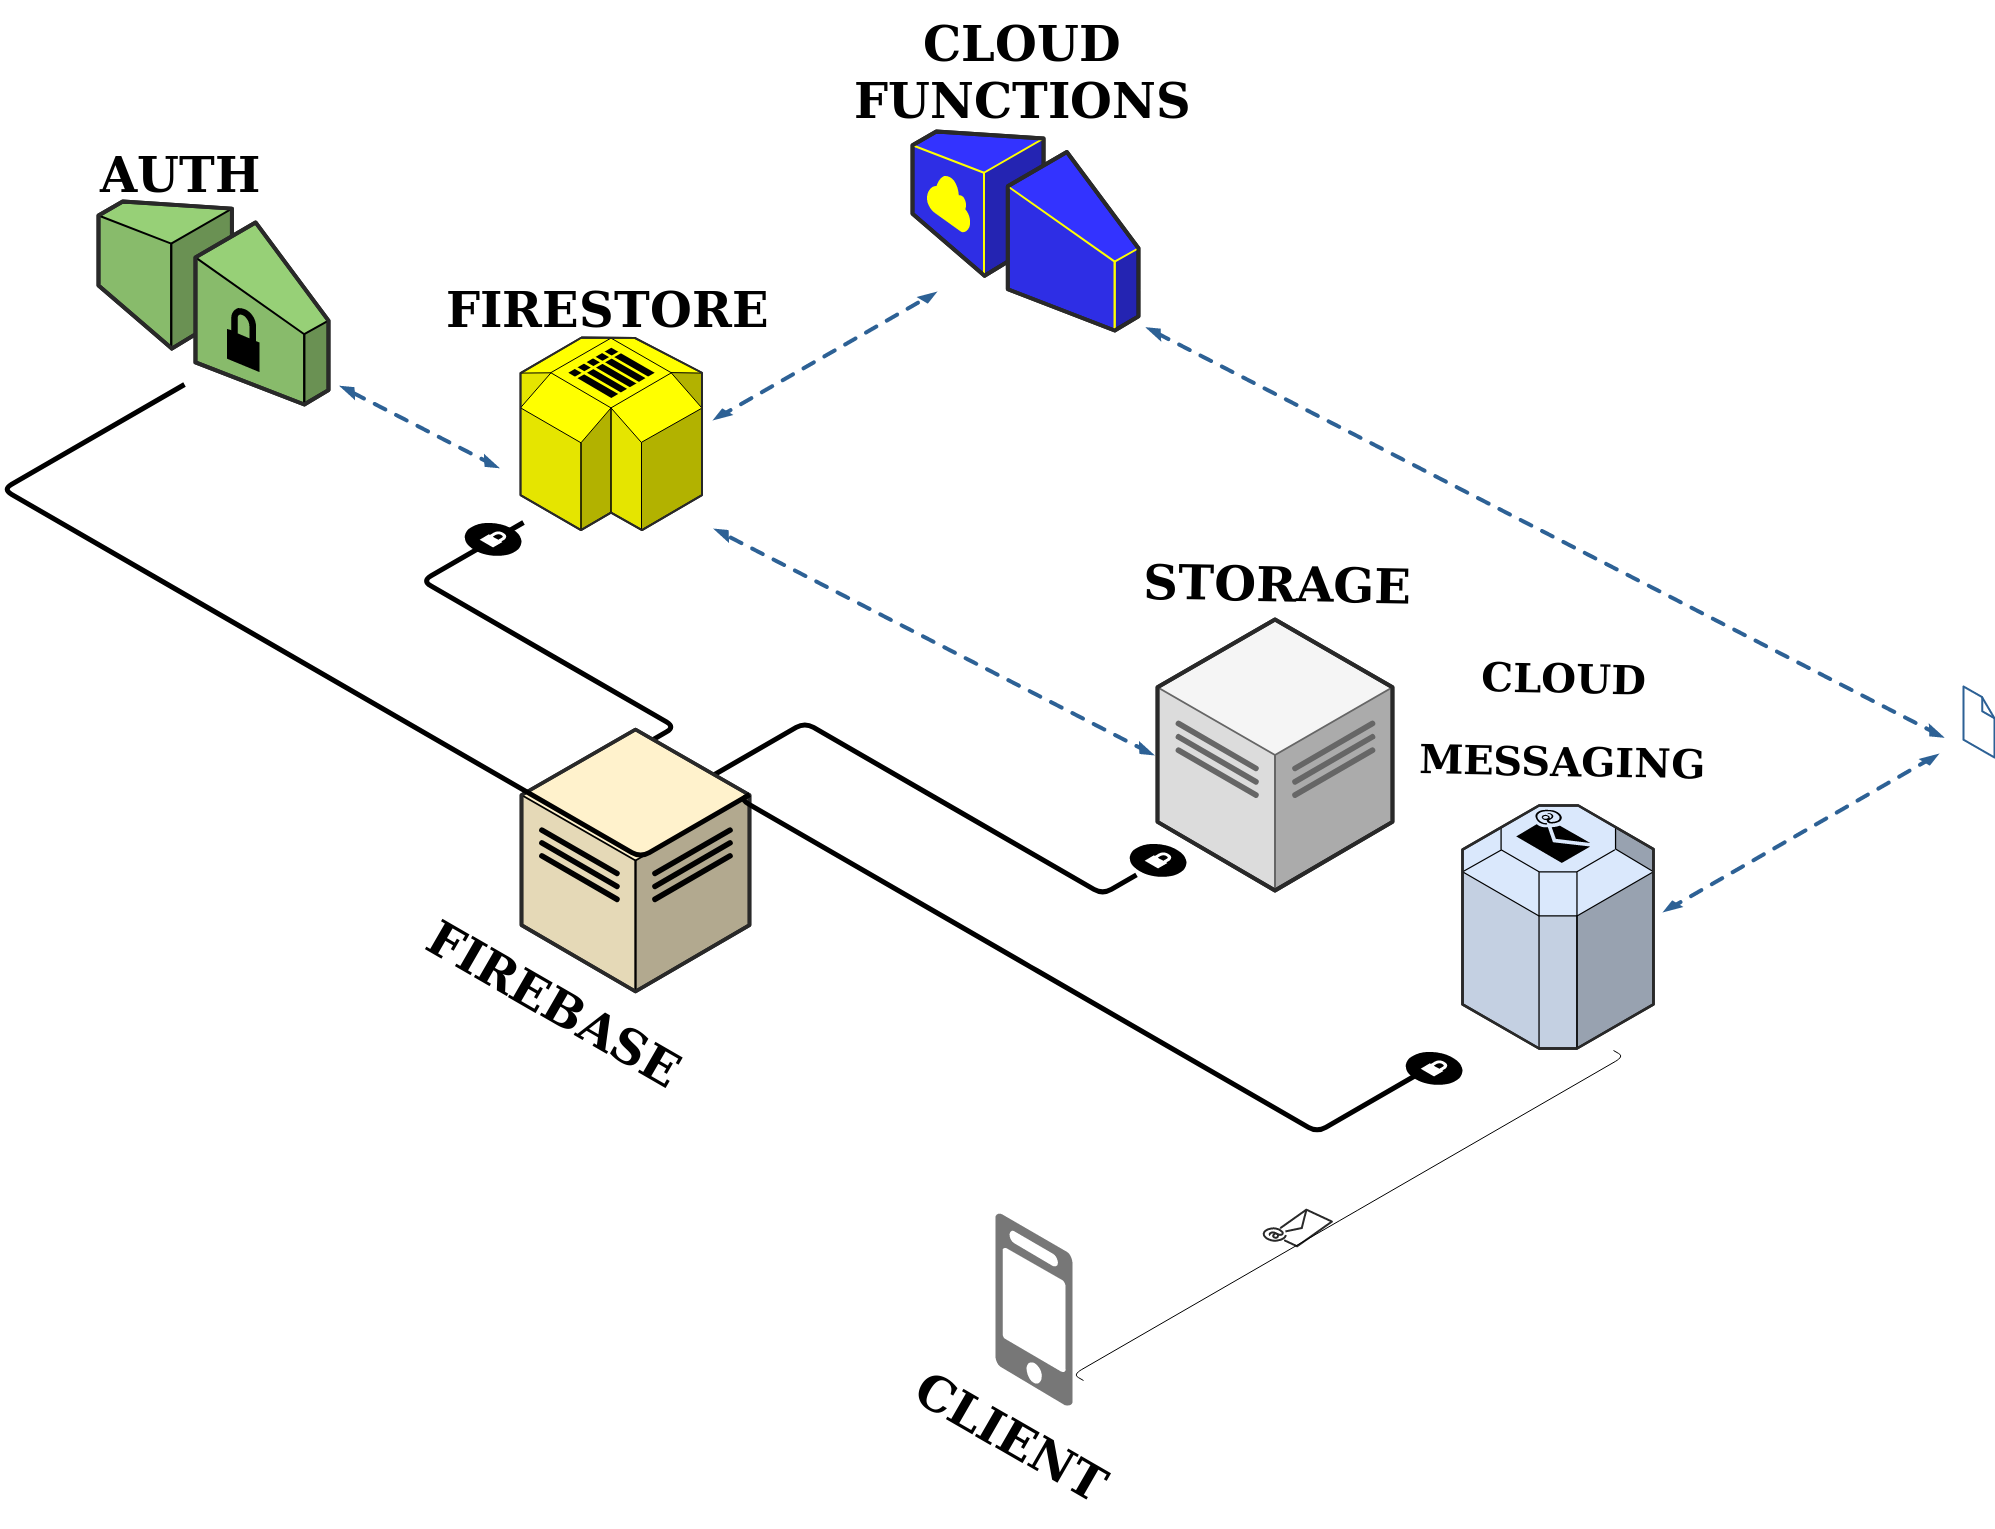
\includegraphics[width=0.8\textwidth]{immagini/server_arch.png}
  \caption{Server Architettura}\label{fig:Architettura Server}
\end{figure}

\subsection{Autenticazione}
I client connessi a Firebase con l'appostia SDK, hanno la possibilit\'a di registrarsi attraverso email, e social login (Google,Faceook,Twitter). Una volta effettuata la registrazione, FirebaseAuth assegner\'a un identificativo univoco al nuovo client, memorizzando nei suoi server le informazioni basilari, quali: ID, nome, data di creazione, ultimo accesso, email, e provider (Email, Google, Faceook, Twitter).
\begin{figure}[!h]
  \centering
  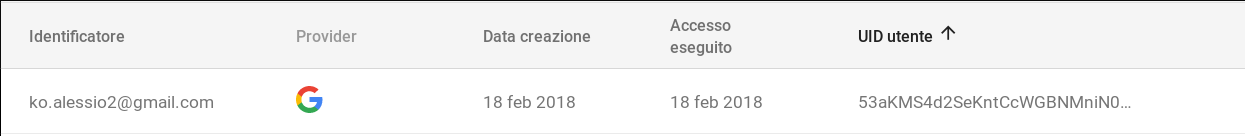
\includegraphics[width=1\textwidth]{immagini/firebase_auth_user.png}
  \caption{Firebase Auth User}\label{fig:Firebase User}
\end{figure}

La parte di autenticazione viene gestita nel file AuthActivity.kt, che controlla se un utente \'e registrato o richiede di registrarsi.
Se l'utente richiede di registrarsi, l'interfaccia e la logica di registrazione vengono controllate dalla libreria FirebaseUI, l'accesso invece viene gestito manualmente.\\
Ogni utente \'e univoco e non pu\'o creare account diversi utilizzando la stessa email, inoltre utilizzando la libreria FirebaseUI si hanno ha disposizione l'integrazione con SmartLock, e l'account linking.
L'account linking consiste nel collegare account che utilizzano la stessa email, se si effettua ad esempio l'accesso attraverso uno dei social supportati, e l'email di registrazione del social \'e gi\'a presente nei server di FirebaseAuth, verr\'a effettuato un collegamento degli account automatico (Account Linking), fra gli account che utilizzano la stessa email.
Quando un utente registrato, effettua l'accesso, viene controllato se \'e presente il record all'interno del database Firestore, in caso contrario viene fatta richiesta di aggiungere il nuovo utente al database Firestore, utilizzando come ID, l'identificativo fornito dal servizio Firebase-Auth.Una volta effettuato l'accesso per evitare ulteriori richieste al Database vengono vengono salvate le informazioni dell'utente e gli identificativi dei membri appartenenti al gruppo nelle "Shared Preferences" di Android.


\subsection{Storage}

Il servizio di storage offerto da Firebase \'e stato utilizzato per salvare le immagini del profilo degli utenti registrati, e le immagini dei gruppi.\\
Il servizio offre la possibilit\'a di inserire qualsiasi tipo di file sia attraverso l'SDK per i vari client sia attraverso il pannello di controllo di Firebase.\\
Ogni file presente sullo storage contiene il nome, la dimensione, il tipo e l'ultima modifica del file, oltre a queste informazioni sono presenti due link: il riferimento del file sullo storage e un URL pubblico che consente il download del file.\\
Il riferimento viene utilizzato dall'SDK per avere un identificativo del file all'interno dello storage e quindi permettere il download del file applicando qual'ora ce ne fosse il bisogno restrizioni sul download, il link pubblico invece permette di visualizzare e scaricare il file a tutti coloro che ne possiedono il link (per motivi di sicurezza questo link pu\'o essere rigenerato).\\
I file sono organizzati in modo da avere le immagini del profilo degli utenti all interno di una cartella separata dalle immagini dei gruppi.\@
Si \'e scelto inoltre di memorizzare i file assegnandoli un identificativo univoco in modo da avere un riferimento di appartenenza sia attraverso il pannello di controllo di Firebase, sia utilizzando l'SDK.\\
Come nome per le immagini profilo, \'e stato usato l'identificativo offerto da FirebaseAuth, come nome per le immagini del gruppo invece \'e stato utilizzato l'identificativo del gruppo assegnato da Firestore.


\subsection{Notifiche}
Le notifiche vengono gestite dal server Cloud Messaging, che si occupa della memorizzazione, invio e ricezioni delle notifiche fra client e server.\\
La ricezione dei messaggi di Cloud Messaging \'e possibile solo se si utilizza l'apposito SDK e si ottiene un token, necessario per inviare un messaggio ad un dispositivo specifico.\\
All'avvio iniziale dell' applicazione, l'SDK FCM genera un token di registrazione per l'istanza dell' applicazione client.\\
I token e la ricezione dei messaggi possono essere controllati utilizzando le classi offerte dall'SDK.
La classe "FirebaseInstanceIdService" viene utilizzata per la gestione dei token, mentre la classe "FirebaseMessagingService" viene utilizzata per la gestione dei messaggi ricevuti.\\
Il token di registrazione pu\'o cambiare quando l'applicazione elimina il token, ripristina,riinstalla, dinistalla l'app, o quando vengono eliminare le cache e i dati dal dispositivo.


\subsection{Database}

\subsection{Cloud Functions}

\section{Client}                 %crea la sezione



\section{Model View Presenter}                 %crea la sezione
MVP (Model View Presenter) \'e un pattern architetturale utilizzato per l'organizzazione strutturale di un progetto, in modo da trarne vantaggio in termini di prestazioni, leggibilit\'a e modularit\'a del codice.\\
La sua caratteristica principale \'e quella di separare il livello di presentazione dalla logica, in modo che tutto ci\'o che riguarda l'interazione dell'utente con l'interfaccia sia separato da come vengono rappresentati i dati.\\
Il pattern MVP deriva dal pattern MVC (Model View Controller), che ha 3 concetti base, che lo definiscono:

\begin{enumerate}
\item Model: Il modello dei dati da visualizzare
\item View: L'interfaccia utente che visualizza i dati
\item Controller: Controlla l'interazione tra Model e View
\end{enumerate}

La principale differenza tra i due pattern \'e che il Presenter del MVP gestisce la logica tra la View e il Model, e la sua implementazione permette di gestire l'interfaccia utente ma soprattutto rendere pi\'u comoda l'interazione tra interfaccia utente e i dati.\\


Come il pattern MVC, anche il pattern MVP permette di rendere le View indipendenti dalla gestione dei dati, dividendo la logica dell' applicazione in tre livelli distinti, livelli che possono essere testati separatamente.\\
La possibilit\'a di poter testare i livelli separatamente \'e una delle caratteristiche del MVP.\@


\begin{enumerate}
\item Model: Il modello \'e un' interfaccia che definisce i dati da visualizzare.
\item View: La View \'e un' interfaccia passiva che visualizza i dati (il modello) e instrada i comandi utente (eventi) al Presenter per agire su tali dati.
\item Presenter: Il Presenter agisce sul modello e sulla vista. Recupera i dati dai repository (il modello) e li formatta per la visualizzazione nella vista.
\end{enumerate}

\begin{figure}[!h]
  \centering
  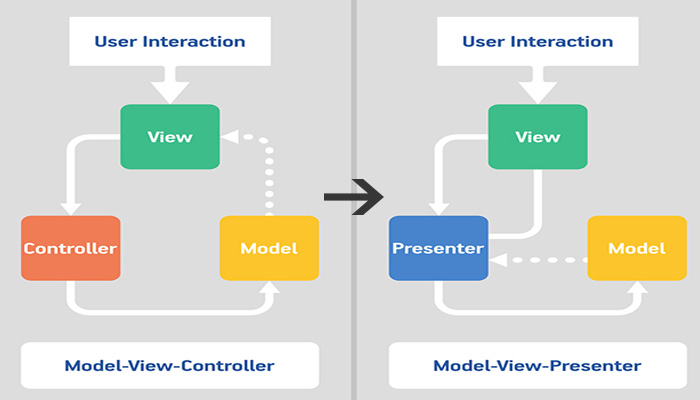
\includegraphics[width=0.65\textwidth]{immagini/mvc-vs-mvp.jpg}
  \caption{MVC vs MVP.}\label{fig:MVC vs MVP}
\end{figure}

\newpage


\subsection{Model}
Il Model \'e un'interfaccia dedicata all'acceso dei dati di un'applicazione, si occupa quindi di fornire un'astrazione del modello dei dati presenti nel database.\\
Il Model oltre a contenere la struttura dei dati da visualizzare si occupa anche di fornire una buona astrazione dei dati presenti nel database, modificando, aggiungendo e separando alcuni dei dati, in modo da rendere l'accesso e la visualizzazione dei dati pi\'u semplice per gli altri due componenti del pattern (View, Presenter).\\
Un esempio potrebbe essere il seguente:
Il database contiene una tabella con due tipi di dato:

\begin{enumerate}
\item \textbf{Nome}: String
\item \textbf{DataDiNascita}: Date
\end{enumerate}

Quando il programma ricever\'a i dati dal database in un qualsiasi formato( Map, Json, Array..) il Model selezionerà i dati in base alla definizione data dal programmatore trasformando il risultato del database in un oggetto.
Questo oggetto oltre a conserare le due informazioni ricevute dal database (Nome, DataDiNascita) potr'\a contenere ance informazioni aggiuntive inserite dal Model per facilitare l'uso e la manipolazione degli altri due componeti.
In questo caso il modello potrebbe creare il nuovo campo "et\'a" facendo una semplice sottrazione fra due date, quella attuale e la data di nascita dell'utente.

\begin{enumerate}
\item \textbf{Nome}: String
\item \textbf{DataDiNascita}: Date
\item \textbf{Et\'a}: Int
\end{enumerate}

%https://medium.com/@cervonefrancesco/model-view-presenter-android-guidelines-94970b430ddf

\subsection{View}
La View \'e un' interfaccia che definisce cosa deve implementare il Presenter, affinch\'e possa interagire con l'interfaccia utente.\\
La View interagisce con il Presenter per visualizzare i dati e notifica al Presenter le azioni che compie l'utente nell'interfaccia.\\
La View pu\'o essere implementata da un Activity, un Fragment, o un widget Android, che contengono ProgressBar, TextView, RecyclerView o altri elementi che necessitano di essere aggiornarnati in base a qualche azione dell'utente o cambiamento nel server.\\
Gli aggiornamenti della View possono essere gestiti in due diversi modi:
\begin{itemize}
    \item Passive View
    \item Supervising Controller
\end{itemize}

Nella Passive View, il Presenter aggiorna la vista per applicare i cambiamenti del modello, in questa modalit\'a l'interazione con il Model è gestita esclusivamente dal Presenter, la vista quindi ha un comportamento "passivo" e non è a conoscenza dei cambiamenti nel Model.\\
Ad esempio, se si dispone di un modulo username/password e di un pulsante "Invia", non si scrive la logica di validazione all' interno della View ma all' interno del Presenter. La View infatti dovrebbe solo contenere il nome utente e la password e inviarli al Presenter.

Nel Supervising Controller, la vista interagisce direttamente con il Model per eseguire semplici operazioni di binding dei dati, senza l' intervento del Presenter. Il Presenter aggiorna il Model, e gestissce cambiamenti sulla View solo nei casi pi\'u complessi, ad esempio l'aggiurnameto di un colore in base alle modifiche effettuate su un dato del Model, poich\'e la modifica non prevede una corrispondenza diretta tra la View e il Model
Entrambe le modalit\'a facilitano il testing delle view in Android poich\'e le loro implementazioni riducono al minimo la quantità di logica implementata nella View.

\begin{figure}[!hb]
  \centering
  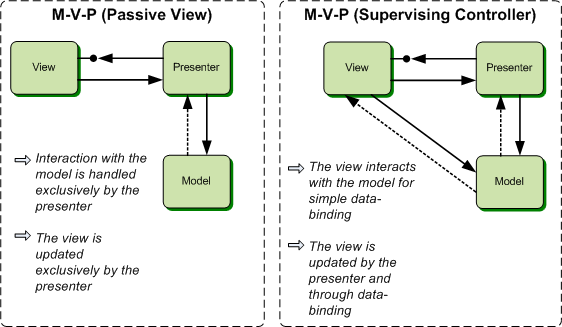
\includegraphics[width=0.7\textwidth]{immagini/mvp_view_types.png}
  \caption{MVP View types}\label{fig:Model View Types}
\end{figure}

\subsection{Presenter}
Il Presenter \'e il mediatore tra il Model e la View e si occupa di  recuperare i dati dal Model, formattarli e passarli alla View, ma a differenza del pattern MVC, decide anche cosa succede quando si interagisce con la View reagendo alle interazioni dell'utente.\\
Il Presenter per facilitare il testing deve cercare di non dipendere minimamente da Android, ma contenere solo metodi e dipendente Java, senza l'utilizzo del "Context" ad esempio, questo permetter\'a di scrivere i test per il Presenter senza l'utilizzo di un emulatore Android.\\
Come detto in precedenza  il Presenter deve dipendere dall' interfaccia View e non direttamente dall' Activity o Fragment, in questo modo si tengono separati il Presenter e l'Activity rispettando la D dei principi SOLID:"Dipendi dalle astensioni. Non dipendere dalle concrezioni"\\





%%%%%%%%%%%%%%%%%%%%%%%%%%%%%%%%%%%%%%%%%non numera l'ultima pagina sinistra
\clearpage{\pagestyle{empty}\cleardoublepage}
